\documentclass{standalone}
\usepackage{pgfplots}
\pgfplotsset{compat=1.17}
\usepackage{amsmath, amssymb, amsbsy, amstext, amsthm, simplewick}
\usepackage{physics}
\usepackage{bm}
\usepackage{siunitx}
\usepackage[acronym]{glossaries}

%% Abbreviations
\newcommand{\eg}{{e.g.}}
\newcommand{\ie}{{i.e.}}

%% Statistics
\newacronym{lbi}{LBI}{likelihood-based inference}
\newacronym{sbi}{SBI}{simulation-based inference}
\newacronym{abc}{ABC}{approximate Bayesian computation}
\newacronym{kl}{KL}{Kullback-Leibler}
\newacronym{vi}{VI}{variational inference}
\newacronym{npe}{NPE}{neural posterior estimation}
\newacronym{nle}{NLE}{neural likelihood estimation}
\newacronym{nre}{NRE}{neural ratio estimation}
\newacronym{mnre}{MNRE}{marginal neural ratio estimation}
\newacronym{tmnre}{TMNRE}{truncated marginal neural ratio estimation}
\newacronym{mcmc}{MCMC}{Markov-chain Monte Carlo}
\newacronym{hmc}{HMC}{Hamiltonian Monte Carlo}
\newacronym{snr}{SNR}{signal-to-noise}
\newacronym{ps}{PS}{power spectrum}
\newacronym{mlr}{MLR}{maximum likelihood ratio}
\newacronym{nn}{NN}{neural network}
\newacronym{cnn}{CNN}{convolutional neural network}
\newacronym{gan}{GAN}{generative adversarial network}
\newacronym{vit}{ViT}{Vision Transformer}
\newacronym{mlp}{MLP}{multilayer perceptron}
\newacronym{bce}{BCE}{binary cross-entropy}

\newcommand{\swyft}{\textit{swyft} }

%% Physics
\newacronym{los}{LOS}{line-of-sight}
\newacronym{nfw}{NFW}{Navarro-Frenk-White}
\newacronym{psf}{PSF}{point-spread function}
\newacronym{shmf}{SHMF}{subhalo mass function}
\newacronym{sie}{SIE}{singular isothermal ellipsoid}
\newacronym{sple}{SPLE}{singular power law ellipsoid}
\newacronym{gr}{GR}{general relativity}
\newacronym{dm}{DM}{dark matter}
\newacronym{cdm}{CDM}{cold dark matter}
\newacronym{wdm}{WDM}{warm dark matter}
\newacronym{hmf}{HMF}{halo mass function}
\newacronym{hst}{HST}{Hubble Space Telescope}


%% Units
\DeclareSIUnit \Mpc {Mpc}
\DeclareSIUnit \arcsec {arcsec}
\DeclareSIUnit \solmass {M_{\odot}}
\newcommand{\keV}{\kiloElectronvolt}

%% Distributions
\newcommand{\Uniform}{\mathcal{U}}
\newcommand{\Normal}{\mathcal{N}}

%% Parameters
\newcommand{\data}{\ensuremath{\bm{x}}}
\newcommand{\param}{\ensuremath{\bm{\Theta}}}
\newcommand{\interest}{\ensuremath{\bm{\theta}}}
\newcommand{\nuisance}{\ensuremath{\bm{\eta}}}

\newcommand{\plens}{\ensuremath{\nuisance_\mathrm{lens}}}
\newcommand{\psrc}{\ensuremath{\nuisance_\mathrm{src}}}
\newcommand{\msub}{\ensuremath{\bm{m}_{200, \mathrm{sub}}}}
\newcommand{\mlos}{\ensuremath{\bm{m}_{200, \mathrm{los}}}}
\newcommand{\psubb}{\ensuremath{{{\nuisance}}_\mathrm{sub}}}
\newcommand{\psub}{\ensuremath{\vec{{\nuisance}}_\mathrm{sub}}}
\newcommand{\plos}{\ensuremath{\vec{{\nuisance}}_\mathrm{los}}}
\newcommand{\pp}{\ensuremath{\boldsymbol{\vec{{\nuisance}}_\mathrm{p}}}}
\newcommand{\zlos}{\ensuremath{\bm{z}_\mathrm{los}}}
\newcommand{\mhm}{\ensuremath{\mathrm{M_{hm}}}}

\newcommand{\hypgeom}{\ensuremath{{}_2\mathrm{F}_1}}

%%%%%%%%%%%%%%%%% Define Lots of Random Colors %%%%%%%%%%%%%%%%%%%%

\definecolor{silver}{rgb}{0.75, 0.75, 0.75}
\definecolor{myblue}{rgb}{0,0.298,0.49}
\definecolor{mauve}{rgb}{0.25, 0.41, 0.88}
\definecolor{red}{rgb}{0.92,0.,0.}
\definecolor{orange}{rgb}{1.0,0.549,0.}
\definecolor{bluegray}{rgb}{0.368417, 0.506779, 0.709798}
\definecolor{lightorange}{rgb}{0.880722, 0.611041, 0.142051}
\definecolor{grassgreen}{rgb}{0.560181, 0.691569, 0.194885}
\definecolor{violet}{rgb}{0.528488, 0.470624, 0.701351}
\definecolor{lightblue}{rgb}{0.363898, 0.618501, 0.782349}
\definecolor{yellow}{rgb}{1, 0.75, 0}
\definecolor{purple}{rgb}{0.647624, 0.37816, 0.614037}
\definecolor{blue}{HTML}{0068AC}
\definecolor{varpurple}{rgb}{0.431,0.188,0.534}
\definecolor{darkgreen}{rgb}{0.075,0.302,0.047}
\definecolor{darkergreen}{rgb}{0,0.294,0.188}
\definecolor{dullred}{rgb}{0.706,0.208,0.192}
\definecolor{darkred}{rgb}{0.545,0,0}
\definecolor{antiquefuchsia}{rgb}{0.57, 0.36, 0.51}
\definecolor{teal}{rgb}{0,0.502,0.502}
\definecolor{dullblue}{rgb}{0,0.298,0.49}
\definecolor{green}{RGB}{44, 160, 44}


\begin{document}

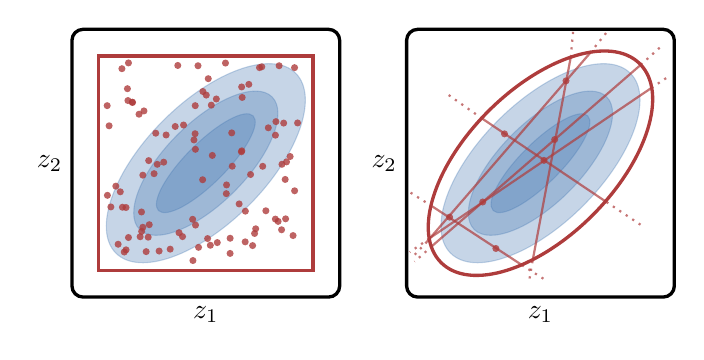
\begin{tikzpicture}[baseline=(current bounding box.center), scale=0.85]

  \pgfmathsetseed{1}

  % Define custom colors
  \definecolor{blue}{RGB}{66, 117, 176}
  \definecolor{red}{RGB}{174, 60, 60}
  % Number of points
  \pgfmathsetmacro{\N}{100}
  % Ellipses
  \draw[opacity=0.3, blue, fill=blue, rotate around={45:(-2,-2)}] (-2,-2) ellipse (1.9 and 0.9);
  \draw[opacity=0.3, blue, fill=blue, rotate around={45:(-2,-2)}] (-2,-2) ellipse (1.4 and 0.6);
  \draw[opacity=0.3, blue, fill=blue, rotate around={45:(-2,-2)}] (-2,-2) ellipse (1 and 0.3);
  % Plot area
  \draw[very thick, line cap=round, rounded corners=4pt] (-4, -4) rectangle (0, 0);
  % Axis labels
  \node[below] at (-2, -4) {$z_1$};
  \node[left] at (-4, -2) {$z_2$};
  % Rectangular box
  \draw[very thick, red] (-3.6, -3.6) rectangle (-0.4, -0.4);
  % Random points
  \foreach \i in {1,...,\N} {
    \pgfmathsetmacro{\x}{-3.5 + rnd * 3.}
    \pgfmathsetmacro{\y}{-3.5 + rnd * 3.}
    \fill[red, opacity=0.8] (\x, \y) circle (1.5pt);
  }
  % Plot area
  \draw[very thick, line cap=round, rounded corners=4pt] (1, -4) rectangle (5, 0);
  % Axis labels
  \node[below] at (3, -4) {$z_1$};
  \node[left] at (1, -2) {$z_2$};
   % Ellipses
  \draw[opacity=0.3, blue, fill=blue, rotate around={45:(3,-2)}] (3,-2) ellipse (1.9 and 0.9);
  \draw[opacity=0.3, blue, fill=blue, rotate around={45:(3,-2)}] (3,-2) ellipse (1.4 and 0.6);
  \draw[opacity=0.3, blue, fill=blue, rotate around={45:(3,-2)}] (3,-2) ellipse (1 and 0.3);
  % Contour
  \draw[very thick, red, rotate around={45:(3,-2)}] (3,-2) ellipse (2.1 and 1.1);
    \pgfmathsetmacro\x{2.93} 
    \pgfmathsetmacro\y{-1.31}
    \fill[red, opacity=0.8, rotate around={45:(3,-2)}] (\x,\y) circle (1.5pt);

    \pgfmathsetmacro\newx{3.067} 
    \pgfmathsetmacro\newy{-2.007}
    \pgfmathsetmacro\m{-0.65}
    \fill[red, opacity=0.8, rotate around={45:(3,-2)}] (\newx,\newy) circle (1.5pt);
    \draw[red, thick, opacity=0.7, rotate around={45:(3,-2)}] (\x-0.075,\y+0.4) -- (\newx+0.22,\newy-1.1);
    \draw[red, thick, opacity=0.7, dotted, rotate around={45:(3,-2)}] (\x-0.18,\y+1) -- (\x-0.075,\y+0.4);
    \draw[red, thick, opacity=0.7, dotted, rotate around={45:(3,-2)}] (\newx+0.22,\newy-1.1) -- (\newx+0.34,\newy-1.7);
    \xdef\x{\newx}
    \xdef\y{\newy}

    \pgfmathsetmacro\newx{1.98} 
    \pgfmathsetmacro\newy{-1.80}
    \fill[red, opacity=0.8, rotate around={45:(3,-2)}] (\newx,\newy) circle (1.5pt);
    \draw[red, thick, opacity=0.7, rotate around={45:(3,-2)}] (\x+1.9,\y-0.37) -- (\newx-0.95,\newy+0.18);
    \draw[red, thick, opacity=0.7, dotted, rotate around={45:(3,-2)}] (\x+1.9,\y-0.37) -- (\x+2.2,\y-0.43);
    \draw[red, thick, opacity=0.7, dotted, rotate around={45:(3,-2)}] (\newx-0.95,\newy+0.18) -- (\newx-1.3,\newy+0.24);
    \xdef\x{\newx}
    \xdef\y{\newy}

    \pgfmathsetmacro\newx{3.4} 
    \pgfmathsetmacro\newy{-1.9}
    \fill[red, opacity=0.8, rotate around={45:(3,-2)}] (\newx,\newy) circle (1.5pt);
    \draw[red, thick, opacity=0.7, rotate around={45:(3,-2)}] (\x-1.,\y+0.07) -- (\newx+1.7,\newy-0.12);
    \draw[red, thick, opacity=0.7, dotted, rotate around={45:(3,-2)}] (\x-1.,\y+0.07) -- (\x-1.35,\y+0.09);
    \draw[red, thick, opacity=0.7, dotted, rotate around={45:(3,-2)}] (\newx+1.7,\newy-0.12) -- (\newx+2.1,\newy-0.14);
    \xdef\x{\newx}
    \xdef\y{\newy}

    \pgfmathsetmacro\newx{4.14} 
    \pgfmathsetmacro\newy{-1.4}
    \fill[red, opacity=0.8, rotate around={45:(3,-2)}] (\newx,\newy) circle (1.5pt);
    \draw[red, thick, opacity=0.7, rotate around={45:(3,-2)}] (\x-1.517,\y-1.05) -- (\newx+0.3,\newy+0.2);
    \draw[red, thick, opacity=0.7, dotted, rotate around={45:(3,-2)}] (\x-1.517,\y-1.05) -- (\x-1.8,\y-1.25);
    \draw[red, thick, opacity=0.7, dotted, rotate around={45:(3,-2)}] (\newx+0.3,\newy+0.2) -- (\newx+0.6,\newy+0.45);
    \xdef\x{\newx}
    \xdef\y{\newy}
    
    \pgfmathsetmacro\newx{1.47} 
    \pgfmathsetmacro\newy{-1.61}
    \fill[red, opacity=0.8, rotate around={45:(3,-2)}] (\newx,\newy) circle (1.5pt);
    \draw[red, thick, opacity=0.7, rotate around={45:(3,-2)}] (\x+0.55,\y+0.04) -- (\newx-0.5,\newy-0.02);
    \draw[red, thick, opacity=0.7, dotted, rotate around={45:(3,-2)}] (\x+0.55,\y+0.04) -- (\x+1,\y+0.09);
    \draw[red, thick, opacity=0.7, dotted, rotate around={45:(3,-2)}] (\newx-0.5,\newy-0.02) -- (\newx-0.8,\newy-0.03);
    \xdef\x{\newx}
    \xdef\y{\newy}

    \pgfmathsetmacro\newx{1.628}
    \pgfmathsetmacro\newy{-2.43}
    \fill[red, opacity=0.8, rotate around={45:(3,-2)}] (\newx,\newy) circle (1.5pt);
    \draw[red, thick, opacity=0.7, rotate around={45:(3,-2)}] (\x-0.07,\y+0.3) -- (\newx+0.1,\newy-0.45);
    \draw[red, thick, opacity=0.7, dotted, rotate around={45:(3,-2)}] (\x-0.07,\y+0.3) -- (\x-0.16,\y+0.7);
    \draw[red, thick, opacity=0.7, dotted, rotate around={45:(3,-2)}] (\newx+0.1,\newy-0.45) -- (\newx+0.2,\newy-0.9);
    \xdef\x{\newx}
    \xdef\y{\newy}

\end{tikzpicture}

\end{document}
